\section{Methodology}
\label{sec:method}

\subsection{Overview of the Proposed Framework}
Figure~\ref{fig:plot} gives an overview. The framework has two stages.

\begin{figure}[t]
  \centering
  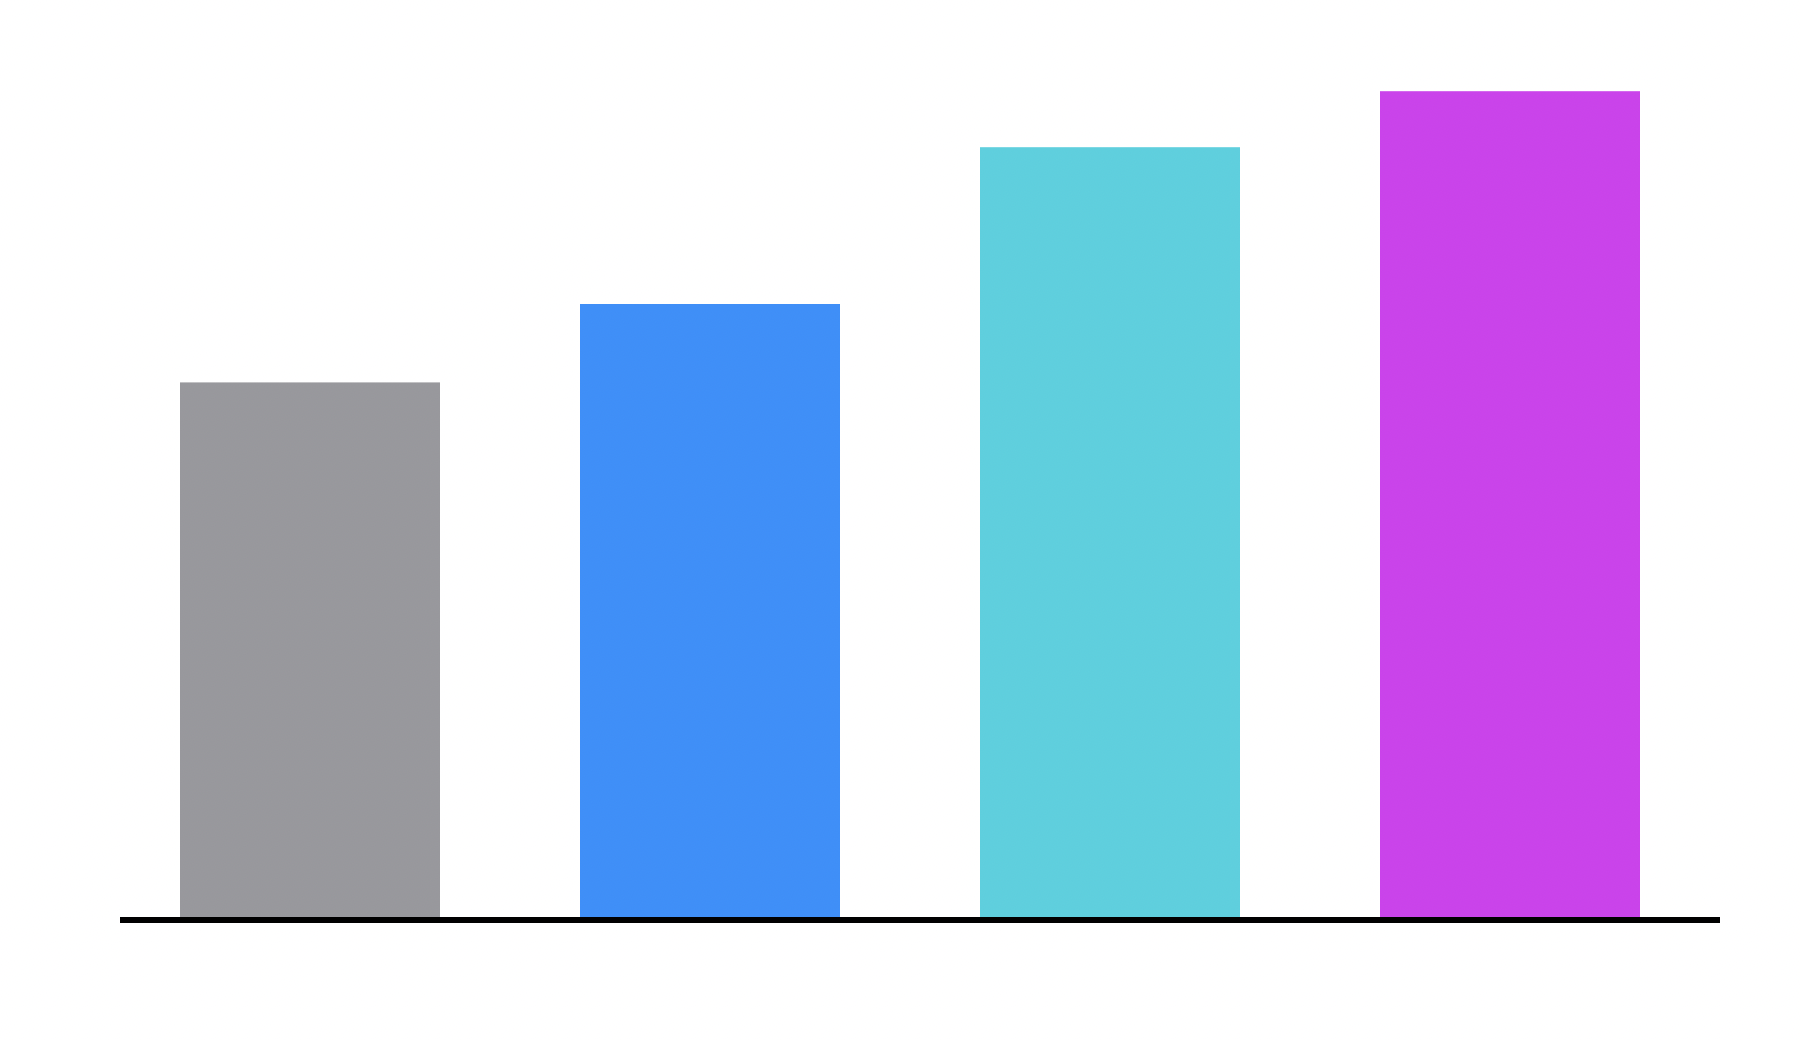
\includegraphics[width=\linewidth]{figures/plot.png}
  \caption{Error reduction of each stage on the validation set.}
  \label{fig:plot}
\end{figure}

\subsection{Notations and Operators}
Let $F$ denote a raw forecast and $O$ the matching observation.

\subsection{Stage 1: Token Codebook}
\subsubsection{Encoder}
The encoder maps the forecast to a latent grid $z = E(F)$.
\subsubsection{Vector Quantization with Dynamic Re-initialization}
Each latent vector is replaced by its nearest codebook entry:
\begin{equation}
  \hat{z}_i = \arg\min_{e_k \in \mathcal{C}} \lVert z_i - e_k \rVert_2 .
  \label{eq:vq}
\end{equation}
\subsubsection{Codebook Training Loss}
We train with the loss in Eq.~\eqref{eq:vq} plus a commitment term.

\subsection{Stage 2: Dual-Path Correction}
\subsubsection{Path 1: Climatology Prior (Fixed)}
A fixed climatology prior supplies seasonal context.
\subsubsection{Path 2: Codebook Tokens $\to$ Correction Head (Trainable)}
A trainable head maps tokens to a residual correction.
